\chapterA{Algoritmo de Prim}
\section{Estructura de archivos}
La carpeta está estructurada de la siguiente manera:
\begin{itemize}
    \item\textbf{bin:} Carpeta que contiene el archivo final de compilación.
    \item\textbf{graph:} Carpeta que contiene los archivos de la biblioteca de grafos y casos de prueba:
    \begin{itemize}
       \item\textbf{graph.h y graph.cpp:} archivos con el código de implementación de grafos mediante listas de adyacencia y el propio algoritmo de Prim.
       \item\textbf{dummygraphs.h:} cabecera que introduce los grafos al programa.
       \item\textbf{test:} carpeta que contiene un generador de grafos aleatorio y los casos de prueba generados
    \end{itemize}
    \item\textbf{obj:} carpeta para la compilación de la librería de grafos.
    \item\textbf{main.cpp}: archivo fuente que corre los casos de prueba.
    \item\textbf{makefile}: archivo make para facilitar la compilación de la práctica.
\end{itemize}

\section{Pruebas}
Todas las pruebas incluyen los tiempos de carga desde archivo de los grafos y la salida por consola del arbol final. Todas las pruebas se realizan en el siguiente sistema:
\begin{itemize}
    \item\textbf{CPU:} i7-8750
    \item\textbf{GPU:} Nvidia Geforce GTX 1060 Mobile
    \item\textbf{RAM:} 16 Gb
    \item\textbf{SO:} ArcoLinux
\end{itemize}



Los gráficos de las pruebas se pueden ver en la figura \ref{fig:prim-plot}~(\nameref{fig:prim-plot})

\begin{figure}[H]
      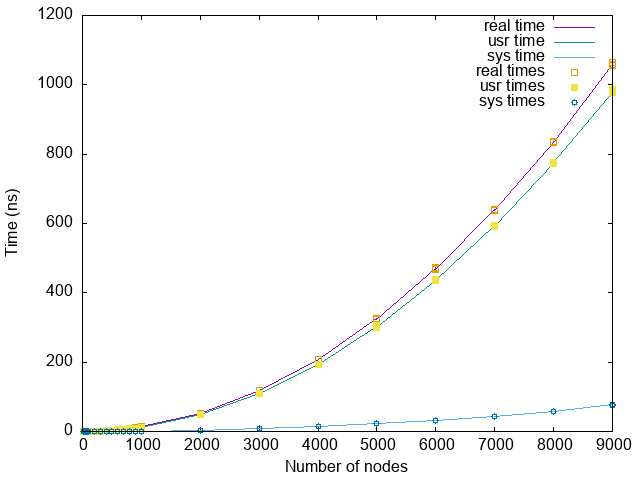
\includegraphics[width = \textwidth]{./images/prim-plot.png}
      \caption{Gráfica de tiempo del algoritmo de Prim para distintas cargas de trabajo.}
      \label{fig:prim-plot}
  \end{figure}


Los tiempos observados se pueden asimilar a las de una función $nlog(n)$, que es lo que se pedría en el enunciado.
A mayor numero de aristas en el grafo, mayor será el coste, pero en el algoritmo implementado si no hay unión (representado por el valor más alto de un int de 32 bits), no se hace ninguna operación y se pasa al siguiente nodo.
